\myslide{Objekte - Übersicht}
{
  \textbf{Aufgabenstellung:}\\[2mm]
  Erweiterung der Sprache \LTWO\ um objektorientierte Konzepte

  \animate{1}
  {
    \begin{itemgroup}{Lösung:}
      \item Einführung einer neuen Sprache \LTWOO
      \item Erweiterung des Scanners und des Parsers
      \item Implementierung neuer Ausdrücke (Methodenaufruf, Objekt, Duplikation und Reihe)
            und Typen (Objekttyp und Reihentyp)
      \item Erweiterung aller Beweiswerkzeuge (Small-Step, ...)
      \item Umbau der internen Strukturen, da diese den neuen Anforderungen
            nicht genügten (z.B. disjunkte Identifier Mengen)
      \item Anpassung von JavaCUP, da der erzeugte Java-Code zu groß war
            und somit nicht mehr kompiliert werden konnte
    \end{itemgroup}
  }
}

\myslide{Objekte - Interne Struktur}
{
  Identifier $id \in Id$ werden in Mengen unterteilt: $x \in Var$, $m \in Method$, $a \in Attribute$ 
  und $self \in Self$. Es wird gefordert, dass diese Mengen disjunkt sein müssen.
  Dazu müssen die Bindungen zwischen den Identifiern bestimmt werden. Folgendes
  Beispiel ist deshalb nicht zulässig:

  \begin{center}
    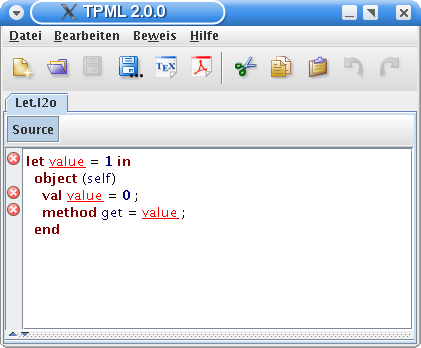
\includegraphics[height=10cm]{images/object_disjunction.png}
  \end{center}
}

\myslide{Objekte - Erweiterung der Produktionen}
{
  \begin{tabular}{lrp{12.0cm}l}
    e      & ::=    & $\Parenthesis{\ExprSend{e}{\ExprIdentifier{m}}}$
                    & \mbox{Methodenaufruf}\\
           & $\mid$ & $\ExprObject{\ExprIdentifier{self}}{\TypeTypeVariable{\tau}}{r}$
                    & \mbox{Objekt}\\
           & $\mid$ & $\ExprDuplication{\ExprIdentifier{$a_1$}\ =\ e_1;\ \ldots\ ; \ExprIdentifier{$a_n$} = e_n}$
                    & \mbox{Duplikation}\\[5mm]

    r      & ::=    & $\ExprRow{\epsilon}$
                    & \mbox{leere Reihe}\\
           & $\mid$ & $\ExprAttribute{\ExprIdentifier{a}}{e}\ r_1$
                    & \mbox{Attribut}\\
           & $\mid$ & $\ExprMethod{\ExprIdentifier{m}}{\TypeTypeVariable{\tau}}{e}\ r_1$
                    & \mbox{Methode}\\[5mm]

    $\tau$ & ::=    & $\TypeObjectType{\TypeRowType{\phi}}$
                    & \mbox{Objekttyp}\\[5mm]

    $\phi$ & ::=    & $\TypeRowType{\emptyset}$
                    & \mbox{Leerer Reihentyp}\\
           & $\mid$ & $\TypeRowType{{\ExprIdentifier{m}}\colon\ {\TypeTypeVariable{\tau}}\ ;}\ \phi_1$
                    & \mbox{Methoden-Reihentyp}
  \end{tabular}
}